% Created by tikzDevice version 0.12.3.1 on 2022-11-04 11:24:38
% !TEX encoding = UTF-8 Unicode
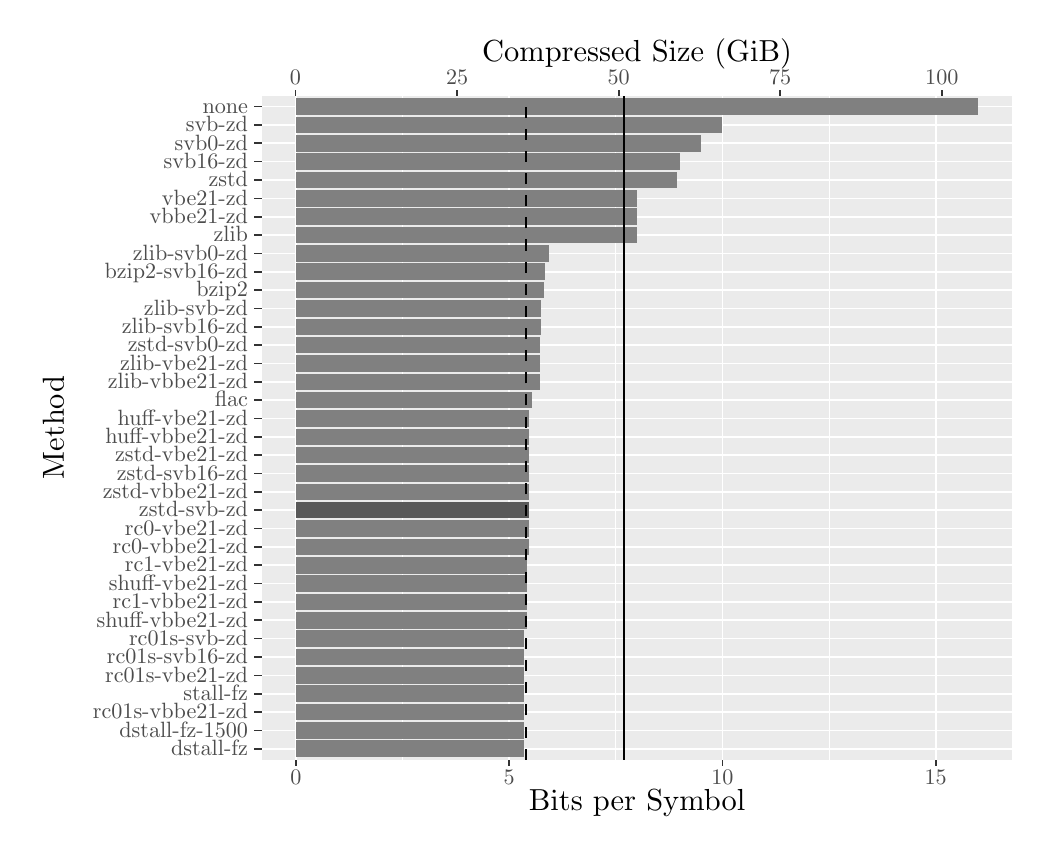
\begin{tikzpicture}[x=1pt,y=0.80pt]
\definecolor{fillColor}{RGB}{255,255,255}
\path[use as bounding box,fill=fillColor,fill opacity=0.00] (0,0) rectangle (361.35,361.35);
\begin{scope}
\path[clip] (  0.00,  0.00) rectangle (361.35,361.35);
\definecolor{drawColor}{RGB}{255,255,255}
\definecolor{fillColor}{RGB}{255,255,255}

\path[draw=drawColor,line width= 0.6pt,line join=round,line cap=round,fill=fillColor] (  0.00,  0.00) rectangle (361.35,361.35);
\end{scope}
\begin{scope}
\path[clip] ( 84.57, 30.69) rectangle (355.85,330.66);
\definecolor{fillColor}{gray}{0.92}

\path[fill=fillColor] ( 84.57, 30.69) rectangle (355.85,330.66);
\definecolor{drawColor}{RGB}{255,255,255}

\path[draw=drawColor,line width= 0.3pt,line join=round] (135.44, 30.69) --
	(135.44,330.66);

\path[draw=drawColor,line width= 0.3pt,line join=round] (212.50, 30.69) --
	(212.50,330.66);

\path[draw=drawColor,line width= 0.3pt,line join=round] (289.57, 30.69) --
	(289.57,330.66);

\path[draw=drawColor,line width= 0.6pt,line join=round] ( 84.57, 35.66) --
	(355.85, 35.66);

\path[draw=drawColor,line width= 0.6pt,line join=round] ( 84.57, 43.94) --
	(355.85, 43.94);

\path[draw=drawColor,line width= 0.6pt,line join=round] ( 84.57, 52.23) --
	(355.85, 52.23);

\path[draw=drawColor,line width= 0.6pt,line join=round] ( 84.57, 60.52) --
	(355.85, 60.52);

\path[draw=drawColor,line width= 0.6pt,line join=round] ( 84.57, 68.80) --
	(355.85, 68.80);

\path[draw=drawColor,line width= 0.6pt,line join=round] ( 84.57, 77.09) --
	(355.85, 77.09);

\path[draw=drawColor,line width= 0.6pt,line join=round] ( 84.57, 85.38) --
	(355.85, 85.38);

\path[draw=drawColor,line width= 0.6pt,line join=round] ( 84.57, 93.66) --
	(355.85, 93.66);

\path[draw=drawColor,line width= 0.6pt,line join=round] ( 84.57,101.95) --
	(355.85,101.95);

\path[draw=drawColor,line width= 0.6pt,line join=round] ( 84.57,110.24) --
	(355.85,110.24);

\path[draw=drawColor,line width= 0.6pt,line join=round] ( 84.57,118.52) --
	(355.85,118.52);

\path[draw=drawColor,line width= 0.6pt,line join=round] ( 84.57,126.81) --
	(355.85,126.81);

\path[draw=drawColor,line width= 0.6pt,line join=round] ( 84.57,135.10) --
	(355.85,135.10);

\path[draw=drawColor,line width= 0.6pt,line join=round] ( 84.57,143.38) --
	(355.85,143.38);

\path[draw=drawColor,line width= 0.6pt,line join=round] ( 84.57,151.67) --
	(355.85,151.67);

\path[draw=drawColor,line width= 0.6pt,line join=round] ( 84.57,159.96) --
	(355.85,159.96);

\path[draw=drawColor,line width= 0.6pt,line join=round] ( 84.57,168.24) --
	(355.85,168.24);

\path[draw=drawColor,line width= 0.6pt,line join=round] ( 84.57,176.53) --
	(355.85,176.53);

\path[draw=drawColor,line width= 0.6pt,line join=round] ( 84.57,184.82) --
	(355.85,184.82);

\path[draw=drawColor,line width= 0.6pt,line join=round] ( 84.57,193.11) --
	(355.85,193.11);

\path[draw=drawColor,line width= 0.6pt,line join=round] ( 84.57,201.39) --
	(355.85,201.39);

\path[draw=drawColor,line width= 0.6pt,line join=round] ( 84.57,209.68) --
	(355.85,209.68);

\path[draw=drawColor,line width= 0.6pt,line join=round] ( 84.57,217.97) --
	(355.85,217.97);

\path[draw=drawColor,line width= 0.6pt,line join=round] ( 84.57,226.25) --
	(355.85,226.25);

\path[draw=drawColor,line width= 0.6pt,line join=round] ( 84.57,234.54) --
	(355.85,234.54);

\path[draw=drawColor,line width= 0.6pt,line join=round] ( 84.57,242.83) --
	(355.85,242.83);

\path[draw=drawColor,line width= 0.6pt,line join=round] ( 84.57,251.11) --
	(355.85,251.11);

\path[draw=drawColor,line width= 0.6pt,line join=round] ( 84.57,259.40) --
	(355.85,259.40);

\path[draw=drawColor,line width= 0.6pt,line join=round] ( 84.57,267.69) --
	(355.85,267.69);

\path[draw=drawColor,line width= 0.6pt,line join=round] ( 84.57,275.97) --
	(355.85,275.97);

\path[draw=drawColor,line width= 0.6pt,line join=round] ( 84.57,284.26) --
	(355.85,284.26);

\path[draw=drawColor,line width= 0.6pt,line join=round] ( 84.57,292.55) --
	(355.85,292.55);

\path[draw=drawColor,line width= 0.6pt,line join=round] ( 84.57,300.83) --
	(355.85,300.83);

\path[draw=drawColor,line width= 0.6pt,line join=round] ( 84.57,309.12) --
	(355.85,309.12);

\path[draw=drawColor,line width= 0.6pt,line join=round] ( 84.57,317.41) --
	(355.85,317.41);

\path[draw=drawColor,line width= 0.6pt,line join=round] ( 84.57,325.69) --
	(355.85,325.69);

\path[draw=drawColor,line width= 0.6pt,line join=round] ( 96.90, 30.69) --
	( 96.90,330.66);

\path[draw=drawColor,line width= 0.6pt,line join=round] (173.97, 30.69) --
	(173.97,330.66);

\path[draw=drawColor,line width= 0.6pt,line join=round] (251.04, 30.69) --
	(251.04,330.66);

\path[draw=drawColor,line width= 0.6pt,line join=round] (328.10, 30.69) --
	(328.10,330.66);
\definecolor{fillColor}{gray}{0.50}

\path[fill=fillColor] ( 96.90,321.96) rectangle (343.52,329.42);

\path[fill=fillColor] ( 96.90,263.96) rectangle (220.12,271.41);

\path[fill=fillColor] ( 96.90,288.82) rectangle (234.61,296.27);

\path[fill=fillColor] ( 96.90,239.10) rectangle (186.58,246.55);

\path[fill=fillColor] ( 96.90,313.68) rectangle (251.05,321.13);

\path[fill=fillColor] ( 96.90,297.10) rectangle (235.63,304.56);

\path[fill=fillColor] ( 96.90,305.39) rectangle (243.48,312.85);

\path[fill=fillColor] ( 96.90,280.53) rectangle (220.24,287.99);

\path[fill=fillColor] ( 96.90,272.24) rectangle (220.23,279.70);
\definecolor{fillColor}{gray}{0.35}

\path[fill=fillColor] ( 96.90,139.66) rectangle (181.12,147.11);
\definecolor{fillColor}{gray}{0.50}

\path[fill=fillColor] ( 96.90,156.23) rectangle (181.12,163.69);

\path[fill=fillColor] ( 96.90,214.24) rectangle (185.30,221.69);

\path[fill=fillColor] ( 96.90,164.52) rectangle (181.13,171.97);

\path[fill=fillColor] ( 96.90,147.94) rectangle (181.12,155.40);

\path[fill=fillColor] ( 96.90,230.81) rectangle (185.50,238.27);

\path[fill=fillColor] ( 96.90,222.52) rectangle (185.42,229.98);

\path[fill=fillColor] ( 96.90,255.67) rectangle (188.34,263.13);

\path[fill=fillColor] ( 96.90,205.95) rectangle (185.29,213.41);

\path[fill=fillColor] ( 96.90,197.66) rectangle (185.28,205.12);

\path[fill=fillColor] ( 96.90,247.38) rectangle (186.82,254.84);

\path[fill=fillColor] ( 96.90,189.38) rectangle (182.14,196.83);

\path[fill=fillColor] ( 96.90,181.09) rectangle (181.15,188.55);

\path[fill=fillColor] ( 96.90,106.51) rectangle (180.57,113.97);

\path[fill=fillColor] ( 96.90,131.37) rectangle (181.05,138.83);

\path[fill=fillColor] ( 96.90,114.80) rectangle (180.58,122.25);

\path[fill=fillColor] ( 96.90, 65.08) rectangle (179.36, 72.53);

\path[fill=fillColor] ( 96.90,172.80) rectangle (181.14,180.26);

\path[fill=fillColor] ( 96.90, 89.94) rectangle (180.55, 97.39);

\path[fill=fillColor] ( 96.90,123.08) rectangle (181.04,130.54);

\path[fill=fillColor] ( 96.90, 98.22) rectangle (180.56,105.68);

\path[fill=fillColor] ( 96.90, 48.50) rectangle (179.35, 55.96);

\path[fill=fillColor] ( 96.90, 56.79) rectangle (179.35, 64.25);

\path[fill=fillColor] ( 96.90, 81.65) rectangle (179.37, 89.11);

\path[fill=fillColor] ( 96.90, 73.36) rectangle (179.37, 80.82);

\path[fill=fillColor] ( 96.90, 31.93) rectangle (179.34, 39.39);

\path[fill=fillColor] ( 96.90, 40.22) rectangle (179.34, 47.67);
\definecolor{drawColor}{RGB}{0,0,0}

\path[draw=drawColor,line width= 0.6pt,line join=round] (215.59, 30.69) -- (215.59,330.66);

\path[draw=drawColor,line width= 0.6pt,dash pattern=on 4pt off 4pt ,line join=round] (179.98, 30.69) -- (179.98,330.66);
\end{scope}
\begin{scope}
\path[clip] (  0.00,  0.00) rectangle (361.35,361.35);
\definecolor{drawColor}{gray}{0.30}

\node[text=drawColor,anchor=base,inner sep=0pt, outer sep=0pt, scale=  0.80] at ( 96.79,335.61) {0};

\node[text=drawColor,anchor=base,inner sep=0pt, outer sep=0pt, scale=  0.80] at (155.18,335.61) {25};

\node[text=drawColor,anchor=base,inner sep=0pt, outer sep=0pt, scale=  0.80] at (213.56,335.61) {50};

\node[text=drawColor,anchor=base,inner sep=0pt, outer sep=0pt, scale=  0.80] at (271.94,335.61) {75};

\node[text=drawColor,anchor=base,inner sep=0pt, outer sep=0pt, scale=  0.80] at (330.32,335.61) {100};
\end{scope}
\begin{scope}
\path[clip] (  0.00,  0.00) rectangle (361.35,361.35);
\definecolor{drawColor}{gray}{0.20}

\path[draw=drawColor,line width= 0.6pt,line join=round] ( 96.79,330.66) --
	( 96.79,333.41);

\path[draw=drawColor,line width= 0.6pt,line join=round] (155.18,330.66) --
	(155.18,333.41);

\path[draw=drawColor,line width= 0.6pt,line join=round] (213.56,330.66) --
	(213.56,333.41);

\path[draw=drawColor,line width= 0.6pt,line join=round] (271.94,330.66) --
	(271.94,333.41);

\path[draw=drawColor,line width= 0.6pt,line join=round] (330.32,330.66) --
	(330.32,333.41);
\end{scope}
\begin{scope}
\path[clip] (  0.00,  0.00) rectangle (361.35,361.35);
\definecolor{drawColor}{gray}{0.30}

\node[text=drawColor,anchor=base east,inner sep=0pt, outer sep=0pt, scale=  0.80] at ( 79.62, 32.63) {dstall-fz};

\node[text=drawColor,anchor=base east,inner sep=0pt, outer sep=0pt, scale=  0.80] at ( 79.62, 40.91) {dstall-fz-1500};

\node[text=drawColor,anchor=base east,inner sep=0pt, outer sep=0pt, scale=  0.80] at ( 79.62, 49.20) {rc01s-vbbe21-zd};

\node[text=drawColor,anchor=base east,inner sep=0pt, outer sep=0pt, scale=  0.80] at ( 79.62, 57.49) {stall-fz};

\node[text=drawColor,anchor=base east,inner sep=0pt, outer sep=0pt, scale=  0.80] at ( 79.62, 65.77) {rc01s-vbe21-zd};

\node[text=drawColor,anchor=base east,inner sep=0pt, outer sep=0pt, scale=  0.80] at ( 79.62, 74.06) {rc01s-svb16-zd};

\node[text=drawColor,anchor=base east,inner sep=0pt, outer sep=0pt, scale=  0.80] at ( 79.62, 82.35) {rc01s-svb-zd};

\node[text=drawColor,anchor=base east,inner sep=0pt, outer sep=0pt, scale=  0.80] at ( 79.62, 90.63) {shuff-vbbe21-zd};

\node[text=drawColor,anchor=base east,inner sep=0pt, outer sep=0pt, scale=  0.80] at ( 79.62, 98.92) {rc1-vbbe21-zd};

\node[text=drawColor,anchor=base east,inner sep=0pt, outer sep=0pt, scale=  0.80] at ( 79.62,107.21) {shuff-vbe21-zd};

\node[text=drawColor,anchor=base east,inner sep=0pt, outer sep=0pt, scale=  0.80] at ( 79.62,115.49) {rc1-vbe21-zd};

\node[text=drawColor,anchor=base east,inner sep=0pt, outer sep=0pt, scale=  0.80] at ( 79.62,123.78) {rc0-vbbe21-zd};

\node[text=drawColor,anchor=base east,inner sep=0pt, outer sep=0pt, scale=  0.80] at ( 79.62,132.07) {rc0-vbe21-zd};

\node[text=drawColor,anchor=base east,inner sep=0pt, outer sep=0pt, scale=  0.80] at ( 79.62,140.35) {zstd-svb-zd};

\node[text=drawColor,anchor=base east,inner sep=0pt, outer sep=0pt, scale=  0.80] at ( 79.62,148.64) {zstd-vbbe21-zd};

\node[text=drawColor,anchor=base east,inner sep=0pt, outer sep=0pt, scale=  0.80] at ( 79.62,156.93) {zstd-svb16-zd};

\node[text=drawColor,anchor=base east,inner sep=0pt, outer sep=0pt, scale=  0.80] at ( 79.62,165.21) {zstd-vbe21-zd};

\node[text=drawColor,anchor=base east,inner sep=0pt, outer sep=0pt, scale=  0.80] at ( 79.62,173.50) {huff-vbbe21-zd};

\node[text=drawColor,anchor=base east,inner sep=0pt, outer sep=0pt, scale=  0.80] at ( 79.62,181.79) {huff-vbe21-zd};

\node[text=drawColor,anchor=base east,inner sep=0pt, outer sep=0pt, scale=  0.80] at ( 79.62,190.07) {flac};

\node[text=drawColor,anchor=base east,inner sep=0pt, outer sep=0pt, scale=  0.80] at ( 79.62,198.36) {zlib-vbbe21-zd};

\node[text=drawColor,anchor=base east,inner sep=0pt, outer sep=0pt, scale=  0.80] at ( 79.62,206.65) {zlib-vbe21-zd};

\node[text=drawColor,anchor=base east,inner sep=0pt, outer sep=0pt, scale=  0.80] at ( 79.62,214.93) {zstd-svb0-zd};

\node[text=drawColor,anchor=base east,inner sep=0pt, outer sep=0pt, scale=  0.80] at ( 79.62,223.22) {zlib-svb16-zd};

\node[text=drawColor,anchor=base east,inner sep=0pt, outer sep=0pt, scale=  0.80] at ( 79.62,231.51) {zlib-svb-zd};

\node[text=drawColor,anchor=base east,inner sep=0pt, outer sep=0pt, scale=  0.80] at ( 79.62,239.79) {bzip2};

\node[text=drawColor,anchor=base east,inner sep=0pt, outer sep=0pt, scale=  0.80] at ( 79.62,248.08) {bzip2-svb16-zd};

\node[text=drawColor,anchor=base east,inner sep=0pt, outer sep=0pt, scale=  0.80] at ( 79.62,256.37) {zlib-svb0-zd};

\node[text=drawColor,anchor=base east,inner sep=0pt, outer sep=0pt, scale=  0.80] at ( 79.62,264.65) {zlib};

\node[text=drawColor,anchor=base east,inner sep=0pt, outer sep=0pt, scale=  0.80] at ( 79.62,272.94) {vbbe21-zd};

\node[text=drawColor,anchor=base east,inner sep=0pt, outer sep=0pt, scale=  0.80] at ( 79.62,281.23) {vbe21-zd};

\node[text=drawColor,anchor=base east,inner sep=0pt, outer sep=0pt, scale=  0.80] at ( 79.62,289.52) {zstd};

\node[text=drawColor,anchor=base east,inner sep=0pt, outer sep=0pt, scale=  0.80] at ( 79.62,297.80) {svb16-zd};

\node[text=drawColor,anchor=base east,inner sep=0pt, outer sep=0pt, scale=  0.80] at ( 79.62,306.09) {svb0-zd};

\node[text=drawColor,anchor=base east,inner sep=0pt, outer sep=0pt, scale=  0.80] at ( 79.62,314.38) {svb-zd};

\node[text=drawColor,anchor=base east,inner sep=0pt, outer sep=0pt, scale=  0.80] at ( 79.62,322.66) {none};
\end{scope}
\begin{scope}
\path[clip] (  0.00,  0.00) rectangle (361.35,361.35);
\definecolor{drawColor}{gray}{0.20}

\path[draw=drawColor,line width= 0.6pt,line join=round] ( 81.82, 35.66) --
	( 84.57, 35.66);

\path[draw=drawColor,line width= 0.6pt,line join=round] ( 81.82, 43.94) --
	( 84.57, 43.94);

\path[draw=drawColor,line width= 0.6pt,line join=round] ( 81.82, 52.23) --
	( 84.57, 52.23);

\path[draw=drawColor,line width= 0.6pt,line join=round] ( 81.82, 60.52) --
	( 84.57, 60.52);

\path[draw=drawColor,line width= 0.6pt,line join=round] ( 81.82, 68.80) --
	( 84.57, 68.80);

\path[draw=drawColor,line width= 0.6pt,line join=round] ( 81.82, 77.09) --
	( 84.57, 77.09);

\path[draw=drawColor,line width= 0.6pt,line join=round] ( 81.82, 85.38) --
	( 84.57, 85.38);

\path[draw=drawColor,line width= 0.6pt,line join=round] ( 81.82, 93.66) --
	( 84.57, 93.66);

\path[draw=drawColor,line width= 0.6pt,line join=round] ( 81.82,101.95) --
	( 84.57,101.95);

\path[draw=drawColor,line width= 0.6pt,line join=round] ( 81.82,110.24) --
	( 84.57,110.24);

\path[draw=drawColor,line width= 0.6pt,line join=round] ( 81.82,118.52) --
	( 84.57,118.52);

\path[draw=drawColor,line width= 0.6pt,line join=round] ( 81.82,126.81) --
	( 84.57,126.81);

\path[draw=drawColor,line width= 0.6pt,line join=round] ( 81.82,135.10) --
	( 84.57,135.10);

\path[draw=drawColor,line width= 0.6pt,line join=round] ( 81.82,143.38) --
	( 84.57,143.38);

\path[draw=drawColor,line width= 0.6pt,line join=round] ( 81.82,151.67) --
	( 84.57,151.67);

\path[draw=drawColor,line width= 0.6pt,line join=round] ( 81.82,159.96) --
	( 84.57,159.96);

\path[draw=drawColor,line width= 0.6pt,line join=round] ( 81.82,168.24) --
	( 84.57,168.24);

\path[draw=drawColor,line width= 0.6pt,line join=round] ( 81.82,176.53) --
	( 84.57,176.53);

\path[draw=drawColor,line width= 0.6pt,line join=round] ( 81.82,184.82) --
	( 84.57,184.82);

\path[draw=drawColor,line width= 0.6pt,line join=round] ( 81.82,193.11) --
	( 84.57,193.11);

\path[draw=drawColor,line width= 0.6pt,line join=round] ( 81.82,201.39) --
	( 84.57,201.39);

\path[draw=drawColor,line width= 0.6pt,line join=round] ( 81.82,209.68) --
	( 84.57,209.68);

\path[draw=drawColor,line width= 0.6pt,line join=round] ( 81.82,217.97) --
	( 84.57,217.97);

\path[draw=drawColor,line width= 0.6pt,line join=round] ( 81.82,226.25) --
	( 84.57,226.25);

\path[draw=drawColor,line width= 0.6pt,line join=round] ( 81.82,234.54) --
	( 84.57,234.54);

\path[draw=drawColor,line width= 0.6pt,line join=round] ( 81.82,242.83) --
	( 84.57,242.83);

\path[draw=drawColor,line width= 0.6pt,line join=round] ( 81.82,251.11) --
	( 84.57,251.11);

\path[draw=drawColor,line width= 0.6pt,line join=round] ( 81.82,259.40) --
	( 84.57,259.40);

\path[draw=drawColor,line width= 0.6pt,line join=round] ( 81.82,267.69) --
	( 84.57,267.69);

\path[draw=drawColor,line width= 0.6pt,line join=round] ( 81.82,275.97) --
	( 84.57,275.97);

\path[draw=drawColor,line width= 0.6pt,line join=round] ( 81.82,284.26) --
	( 84.57,284.26);

\path[draw=drawColor,line width= 0.6pt,line join=round] ( 81.82,292.55) --
	( 84.57,292.55);

\path[draw=drawColor,line width= 0.6pt,line join=round] ( 81.82,300.83) --
	( 84.57,300.83);

\path[draw=drawColor,line width= 0.6pt,line join=round] ( 81.82,309.12) --
	( 84.57,309.12);

\path[draw=drawColor,line width= 0.6pt,line join=round] ( 81.82,317.41) --
	( 84.57,317.41);

\path[draw=drawColor,line width= 0.6pt,line join=round] ( 81.82,325.69) --
	( 84.57,325.69);
\end{scope}
\begin{scope}
\path[clip] (  0.00,  0.00) rectangle (361.35,361.35);
\definecolor{drawColor}{gray}{0.20}

\path[draw=drawColor,line width= 0.6pt,line join=round] ( 96.90, 27.94) --
	( 96.90, 30.69);

\path[draw=drawColor,line width= 0.6pt,line join=round] (173.97, 27.94) --
	(173.97, 30.69);

\path[draw=drawColor,line width= 0.6pt,line join=round] (251.04, 27.94) --
	(251.04, 30.69);

\path[draw=drawColor,line width= 0.6pt,line join=round] (328.10, 27.94) --
	(328.10, 30.69);
\end{scope}
\begin{scope}
\path[clip] (  0.00,  0.00) rectangle (361.35,361.35);
\definecolor{drawColor}{gray}{0.30}

\node[text=drawColor,anchor=base,inner sep=0pt, outer sep=0pt, scale=  0.80] at ( 96.90, 19.68) {0};

\node[text=drawColor,anchor=base,inner sep=0pt, outer sep=0pt, scale=  0.80] at (173.97, 19.68) {5};

\node[text=drawColor,anchor=base,inner sep=0pt, outer sep=0pt, scale=  0.80] at (251.04, 19.68) {10};

\node[text=drawColor,anchor=base,inner sep=0pt, outer sep=0pt, scale=  0.80] at (328.10, 19.68) {15};
\end{scope}
\begin{scope}
\path[clip] (  0.00,  0.00) rectangle (361.35,361.35);
\definecolor{drawColor}{RGB}{0,0,0}

\node[text=drawColor,anchor=base,inner sep=0pt, outer sep=0pt, scale=  1.10] at (220.21,346.14) {Compressed Size (GiB)};
\end{scope}
\begin{scope}
\path[clip] (  0.00,  0.00) rectangle (361.35,361.35);
\definecolor{drawColor}{RGB}{0,0,0}

\node[text=drawColor,anchor=base,inner sep=0pt, outer sep=0pt, scale=  1.10] at (220.21,  7.64) {Bits per Symbol};
\end{scope}
\begin{scope}
\path[clip] (  0.00,  0.00) rectangle (361.35,361.35);
\definecolor{drawColor}{RGB}{0,0,0}

\node[text=drawColor,rotate= 90.00,anchor=base,inner sep=0pt, outer sep=0pt, scale=  1.10] at ( 13.08,180.68) {Method};
\end{scope}
\end{tikzpicture}
